\subsubsection{React}

\subsubsection*{Správa stavů, předávání vlastností}

Při implementaci jednoduchého čítače začneme tím, že vytvoříme Counter komponentu. Ta bude mít stav \emph{count} a~setter \emph{setCount} pro tento stav.

\begin{prog}
// Část souboru Counter.tsx

function Counter() \{
  const [count, setCount] = useState(0);
\}

export default Counter;
\end{prog}

Naprogramujeme komponentu Button kvůli principu DRY a~celkově znovupoužitelnosti kódu. 
Typ \emph{ButtonProps} obsahuje vlastnosti, které můžeme tlačítku předat -- \emph{className}, \emph{onClick} a~\emph{children}. 
Díky tomu, že typ rozšiřuje \emph{ButtonHTMLAttributes<HTMLButtonElement>}, můžeme předat do komponenty i~další běžné atributy HTML tlačítek (např.~type, value, disabled).

\begin{prog}
// Část souboru Button.tsx

interface ButtonProps extends ButtonHTMLAttributes<HTMLButtonElement> \{
  className: string;
  onClick: () => void;
  children: ReactNode;
\}
\end{prog}

V~rámci argumentu Button komponenty použijeme ES6 destructuring assignment pro získání vlastností. 
Z~objektu vlastností získáme \emph{className} a~\emph{children}, ostatní vlastnosti ponecháme zabalené v~proměnné props pomocí spread operátoru. 
Nyní můžeme vytvořit JSX pro samotné tlačítko. Vlastnost \emph{className} přidáme do tříd tlačítka. 
Pomocí \emph{children} můžeme do tlačítka vložit libovolný obsah, který bude mezi párovými značkami <Button>. 
Všechny ostatní vlastnosti pomocí spread operátoru předáme přímo tlačítku.

\begin{prog}
// Část souboru Button.tsx

function Button(\{className, children, ...props\}: ButtonProps): JSX.Element \{
  return (
    <button
      type="button"
      className=\{`px-4 py-2 rounded-md focus:outline-none \$\{className\}`\}
      \{...props\}
    >
      \{/* children slouží k vykreslení obsahu, 
        který vložíme mezi párové tagy dané komponenty. */\}
      \{children\}
    </button>
  );
\}

export default Button;
\end{prog}

V~Counter komponentě uvnitř JSX vrátíme hodnotu stavu \emph{count} a~vykreslíme Button komponenty, jimž předáme potřebné vlastnosti. 
Pro aktualizaci stavu využijeme vlastnost \emph{onClick}, které předáme anonymní funkci (arrow function) a~v~ní zavoláme \emph{setCount}.

\begin{prog}
// Část souboru Counter.tsx

function Counter() \{
  const [count, setCount] = useState(0);

  return (
    <div className="bg-gray-200 p-6 rounded-md shadow-md">
      <p className="text-xl font-semibold mb-4">Current count: \{count\}</p>

      <div className="flex gap-4">
        <Button
          className="bg-blue-500 text-white hover:bg-blue-600"
          onClick=\{() => setCount(count + 1)\}
        >
          Increment
        </Button>

        \{/* Další komponenty Button... */\}
      </div>
    </div>
  );
\}
\end{prog}

\subsubsection*{Interakce v uživatelském prostředí}

Pro vytvoření jakékoliv UI komponenty můžeme začít tvořit jak JSX, definici komponenty, nebo znovupoužitelný hook. 
V~tomto případě, při vývoji komponenty rozevíracího seznamu, začneme naprogramováním vlastního hooku, který se odděleně postará o~veškerou logiku seznamu.

Hook \emph{useDropdown} bude mít 2 parametry -- obslužnou funkci ke změně vybrané možnosti v~rodičovské komponentě (\emph{onChange}) a~výchozí hodnotu vybrané možnosti (\emph{defaultValue}). 
V~hooku nadefinujeme stavy \emph{selectedOption}, \emph{isOpen} a~vygenerujeme unikátní identifikátor. 
Dále vytvoříme funkci \emph{handleOptionClick}, která zajistí změnu vybrané možnosti, zavření seznamu a~vypublikuje změnu hodnoty do rodičovské komponenty. 
Z~hooku vracíme potřebné stavy a~funkce ve formě objektu nebo pole -- pole musíme označit jako \emph{const}.

\begin{prog}
// Část souboru useDropdown.ts

function useDropdown(
  onChange: (selectedOption: Option | null) => void,
  defaultValue: Option | null,
) \{
  const [selectedOption, setSelectedOption] 
    = useState<Option | null>(defaultValue);
  const [isOpen, setIsOpen] = useState(false);

  // Toto ID je třeba nastavit na kořenový element dropdown komponenty.
  const dropdownId = `id-\$\{crypto.randomUUID()\}`;

  // Obslužná funkce, která se stará o logiku
    po kliknutí na jednotlivé položky v dropdownu.
  const handleOptionClick = (option: Option) => \{
    setSelectedOption(option);
    setIsOpen(false);
    onChange(option);
  \};

  // Vrátíme všechny hodnoty, které chceme mít dostupné zvenčí.
  return [dropdownId, selectedOption, 
    isOpen, setIsOpen, handleOptionClick] as const;
\}
\end{prog}

Pokračujeme tvorbou JSX komponenty Dropdown, kde vložíme tlačítko a~seznam možností. Otevření možností zajistíme přidáním \emph{onClick} (což je vlastně \emph{MouseEventHandler}). 
V~anonymní funkci pak změníme stav pomocí \emph{isOpen} na opačnou hodnotu. Abychom předešli event bubblingu, v~anynomní obslužné funkci zavoláme \emph{event.stopPropagation()}.

\begin{prog}
// Část souboru Dropdown.tsx

<div className="rounded-md shadow-sm">
  \{/* Pro poslouchání na události v DOMu můžeme použít syntaxi: 
    NÁZEV_UDÁLOSTI=\{OBSLUŽNÁ_METODA\}. */\}
  <button
    type="button"
    className=\{`STATICKÉ STYLY... \$\{sizeStyles\} \$\{buttonStyles\}`\}
    onClick=\{event => \{
      event.stopPropagation();
      setIsOpen(!isOpen);
    \}\}
  >
    \{selectedOption ? selectedOption.label : placeholder\}
    \{isOpen ? arrowUpIcon : arrowDownIcon\}
  </button>
</div>
\end{prog}

Seznam možností zobrazíme podmíněně na základě stavu \emph{isOpen}. Pro vykreslení možností seznamu (\emph{options}) použijeme JavaScriptovou funkci \emph{map} uvnitř JavaScriptové hodnoty v~JSX. 
V~Reactu je důležité vždy při použití funkce \emph{map} nastavit unikátní klíč (\emph{key}) pro každou položku v~seznamu. Tento klíč slouží k~identifikaci jednotlivých prvků a~optimalizaci procesu renderování. 
Pro vybrání konkrétní možnosti použijeme \emph{onClick}, kterému předáme anonymní funkci. V~anonymní funkci zavoláme funkci \emph{handleOptionClick} hooku \emph{useDropdown} s~aktuální položkou ze seznamu.

\begin{prog}
// Část souboru Dropdown.tsx

\{isOpen && (
  <div className=\{`STATICKÉ STYLY... \$\{divStyles\}`\}>
    <div
      className="py-1"
      role="menu"
      aria-orientation="vertical"
      aria-labelledby="options-menu"
    >
      \{/* Pro vykreslení seznamu (listu) můžeme využít bloky \{ \}
       a JavaScriptovou funkci .map(). */\}
      \{options.map(option => (
        <button
          key=\{option.value\}
          className=\{`STATICKÉ STYLY... \$\{optionStyles\}`\}
          role="menuitem"
          onClick=\{() => handleOptionClick(option)\}
        >
          \{option.label\}
        </button>
      ))\}
    </div>
  </div>
)\}
\end{prog}

Abychom uzavřeli jakýkoli aktuálně otevřený rozbalovací seznam na stránce, po kliknutí mimo tento seznam, předáme kořenovému elementu dříve vytvořený unikátní identifikátor. 
Do \emph{useDropdown} přidáme \emph{useEffect} a~díky němu budeme naslouchat na události pointerdown v~DOM. Obslužná funkce pak zajistí zavření aktuálně otevřeného dropdownu.

\begin{prog}
// Část souboru useDropdown.ts

useEffect(() => \{
  // Obslužná funkce handleClickOutsideDropdown zajistí zavření dropdownu,
    pokud uživatel klikne mimo něj.
  const handleClickOutsideDropdown = (\{target\}: PointerEvent) => \{
    if (!(target as HTMLElement).closest(`#\$\{dropdownId\}`)) \{
      setIsOpen(false);
    \}
  \};

  // Přidáme posluchač události na událost pointerdown a jeho obslužnou funkci.
  document.addEventListener('pointerdown', handleClickOutsideDropdown);

  // Funkce, která se zavolá při odpojení komponenty.
  return () => \{
    // Odebereme posluchač události na událost
      pointerdown a jeho obslužnou funkci.
    document.removeEventListener('pointerdown', handleClickOutsideDropdown);
  \};
  // Druhý parametr useEffectu je pole závislostí, 
    které určuje, kdy se má useEffect spustit.
\}, [dropdownId]);
\end{prog}

Dropdown samozřejmě může mít i~jiné vstupy, které povedou k~lepší znovupoužitelnosti. 
Dynamické CSS třídy ve formě JavaScriptu na element přidáme pomocí šablonových literálů (template literals) a~JS hodnoty.

\subsubsection*{Reaktivita, asynchronní operace}

Následující komponenta bude demonstrovat využití reaktivity a~asynchronních operací. Vytvoříme komponentu, která přeloží zadaný text do cílového jazyka. 
Začneme implementací komponenty Translator. Komponenta při změně stavů (zadaného textu uživatelem a~výstupního jazyka) zavolá API, které vrátí přeložený text.
Uvnitř komponenty vykreslíme vnořené komponenty pro zadání vstupního textu, výběr jazyka a~zobrazení výsledku.

Komponenta LanguageDropdown uživateli umožní vybrat jazyk, do kterého chce text přeložit. 
Díky vlastnosti \emph{onChange} (callback funkci) aktualizujeme výstupní jazyk v~rodičovské komponentě. 

Pokračujeme implementací komponenty TranslationInput, která bude sloužit k~zadání vstupního textu přes textové pole. Aktuální hodnotu formulářového prvku nastavíme pomocí atributu \emph{value}.
Po změně hodnoty textového pole, kterou získáme v~události přes atribut \emph{onChange}, aktualizujeme hodnotu vstupního textu v~Translator komponentě.

\begin{prog}
// Část souboru TranslationInput.tsx

<textarea
  ref=\{textAreaRef\}
  className="block w-full min-h-0 p-3 pr-12 pb-8 resize-none !outline-none"
  placeholder="Type to translate ..."
  value=\{inputText\}
  onChange=\{handleInputChange\}
/>
\end{prog}

Abychom reaktivně aktualizovali výšku pole na základě obsahu, použijeme vlastní hook. 
Hook bude potřebovat referenci elementu, a~tak vytvoříme ref, který přidáme na element textového pole.

\begin{prog}
// Část souboru TranslationInput.tsx

function TranslationInput(\{inputText, setInputText\}: TranslationInputProps) \{
  // Vytvoření reference pro textovou oblast.
  const textAreaRef = useRef<HTMLTextAreaElement>(null);

  // Použití vlastního hooku pro automatickou aktualizaci výšky
    textové oblasti na základě reference.
  useAutosizeTextArea(textAreaRef.current, inputText);

  return (
    \{/* JSX... */\}
  );
\}
\end{prog}

Hook \emph{useAutosizeTextArea} bude příjímat referenci na element. Dále také hodnotu textového pole, aby se po jakékoli změně této hodnoty přepočítala výška pole. 
Do hooku přidáme \emph{useEffect}, který se znovu zavolá při každé změně \emph{textAreaRef}, nebo hodnoty textu. V~neposlední řadě aktualizujeme výšku textového pole.

\begin{prog}
// Část souboru useAutoresizeTextarea.ts

const useAutosizeTextArea = (
  textAreaRef: HTMLTextAreaElement | null, value: string
) => \{
  useEffect(() => \{
    if (textAreaRef) \{
      // Abychom získali správnou výšku scrollHeight 
        pro textovou oblast, musíme výšku resetovat.
      textAreaRef.style.height = '0px';

      // Výšku pak nastavíme přímo na nativní prvek.
      // Při pokusu o nastavení této hodnoty pomocí stavu 
        nebo odkazu bude výsledkem nesprávná hodnota.
      textAreaRef.style.height = `\$\{textAreaRef.scrollHeight + 36\}px`;
    \}
  \}, [textAreaRef, value]);
\};
\end{prog}

V~Translator komponentě potřebujeme ukládat vstupní hodnotu a~výstupní jazyk z~vnořených komponent. 
Dále při každé změně těchto hodnot odešleme dotaz na Microsoft Translator Text API \cite{translatortextapi}, k~čemuž využijeme \emph{useEffect}.
V~rámci hooku definujeme asynchronní funkci \emph{handleTranslation}, která pomocí fetch API odešle korektní HTTP POST požadavek na server. 
Pokud bychom definovali funkci mimo \emph{useEffect}, museli bychom ji přidat do pole závislostí hooku.
Při úspěšné odpovědi aktualizujeme stav s~přeloženým textem, v~opačném případě nastavíme chybový stav.

\begin{prog}
// Část souboru Translator.tsx

useEffect(() => \{
  // Funkce pro zpracování přeložení textu.
  const handleTranslation = async () => \{
    if (!inputText.length) return;

    // Zrušení předchozího asynchronního požadavku.
    abortControllerRef.current?.abort();
    // Vytvoření nového kontroleru pro zrušení asynchronního požadavku.
    abortControllerRef.current = new AbortController();
    setLoading(true);

    const parsedInputText = inputText.replace(/\verb"\n"/g, '');
    const url = `\$\{import.meta.env.VITE_RAPID_API_BASE_URL\}\$\{outputLanguage\}\$\{
      import.meta.env.VITE_RAPID_API_QUERY_PARAMS
    \}`;
    const options = \{
      method: 'POST',
      headers: \{
        'content-type': 'application/json',
        'X-RapidAPI-Key': import.meta.env.VITE_RAPID_API_KEY,
        'X-RapidAPI-Host': 'microsoft-translator-text.p.rapidapi.com',
      \},
      body: `[\{"Text":"\$\{parsedInputText\}"\}]`,
      signal: abortControllerRef.current?.signal,
    \};

    try \{
      // Odeslání HTTP POST požadavku na server, 
        který nám vrátí přeložený text v nějaké struktuře.
      const response = await fetch(url, options);

      if (!response.ok) \{
        throw new Error(
          `Something went wrong: \$\{response.status\} Error.
          Please reload the page.`,
        );
      \}

      const result = await response.json();
      const translatedText = result[0].translations[0].text as string;
      setOutputText(translatedText);
      // eslint-disable-next-line @typescript-eslint/no-explicit-any
    \} catch (error: any) \{
      // Pokud je chyba typu AbortError, tak ji ignorujeme.
      if (error.name === 'AbortError') return;

      setError(error);
    \} finally \{
      setLoading(false);
    \}
  \};

  // Zrušení předchozího časovače.
  clearTimeout(delayTimerRef.current);

  // Zpoždění překladu o 300 ms.
  delayTimerRef.current = setTimeout(() => handleTranslation(), 300);

  // Zrušení časovače při zničení komponenty.
  return () => clearTimeout(delayTimerRef.current);
\}, [inputText, outputLanguage]);
\end{prog}

Aby dotazování fungovalo, vytvoříme referenci \emph{delayTimerRef}. V~rámci těla \emph{useEffect} hooku nejprve zrušíme předchozí časovač. 
Funkci \emph{handleTranslation} zavoláme v~callbacku funkce \emph{setTimeout}, která umožní předejít dotazování serveru ihned po změně nějaké vstupní hodnoty. 
Výsledek funkce \emph{setTimeout} uložíme do \emph{delayTimerRef.current}. Nesmíme také zapomenout na zrušení časovače při zničení komponenty.

V~okamžiku, kdy obdržíme odpověď ze serveru, zobrazíme přeložený text uživateli pomocí komponenty TranslationOutput. 
Předáme jí samotný výstupní text a~další vstupní vlastnosti, na základě kterých pak podmíněně vykreslíme přeložený text, chybu nebo načítání.

\subsubsection*{Tvorba formulářů, validace}

React sám o~sobě poskytuje jen základní API pro správu formulářů. Disponuje však mnoha knihovnami, které tuto funkcionalitu rozšiřují. 
Mezi takové knihovny patří např.~Formik, Redux Form nebo React Hook Form. V~této sekci se zaměříme na tvorbu formulářů pomocí React Hook Form \cite{reacthookformlib}. 
Vytvoříme komponentu InvestForm pro jednoduchou investiční kalkulaci. 
V~této komponentě naprogramujeme formulář pro zadání vstupních dat a~komponentu výsledku kalkulace, která se zobrazí po potvrzení formuláře.

Začneme s~reaktivním fomulářem, který bude přijímat počáteční hodnoty (\emph{defaultValues}) a~callback funkci \emph{handleFormSubmit} pro předání hodnot formuláře do rodičovské komponenty. 
Strukturu formuláře popíšeme v~typu \emph{InvestFormData}. Pomocí hooku \emph{useForm} z~knihovny React Hook Form vytvoříme instanci formuláře, které předáme \emph{defaultValues} a~nastavíme reaktivní validaci. 
Následně z~hooku dostameme funkce \emph{register}, \emph{handleSubmit} a~\emph{formState}, které poslouží ke správě formuláře.

\begin{prog}
// Část souboru types.ts

export interface InvestFormData \{
  oneOffInvestment: number;
  investmentLength: number;
  averageSavingsInterest: number;
  averageSP500Interest: number;
\}

// Část souboru InvestForm.tsx

const \{
  register,
  handleSubmit,
  formState: \{errors\},
\} = useForm<InvestFormData>(\{defaultValues, mode: 'onChange'\});
\end{prog}

Do JSX přidáme form značku s~\emph{onSubmit} atributem, kterému předáme funkci \emph{handleSubmit} z~React Hook Form. Do \emph{handleSubmit} pak vložíme vstup \emph{handleFormSubmit} v~němž získáme aktuální hodnoty formuláře. 
Ve formuláři vytvoříme formulářové prvky, které propojíme s~reaktivním formulářem pomocí funkce \emph{register}. První argument představuje název formulářového prvku, druhý argument je validační objekt. 
V~rámci range inputu potřebujeme HTML atributy min a~max, díky kterým omezíme rozsah vstupních hodnot. Abychom měli přístup k~aktuální hodnotě range inputu, využijeme vlastnost \emph{value} a~\emph{onChange}. 
Chyby formuláře získáme z~\emph{formState} a~vykreslíme je pod formulářovými prvky. V~neposlední řadě přidáme tlačítko s~typem submit, které zajistí odeslání formuláře a~zavolání callback funkce \emph{handleFormSubmit}.

\begin{prog}
// Část souboru InvestForm.tsx

return (
  <form onSubmit={handleSubmit(handleFormSubmit)}>
    <div className="md:flex md:gap-4">
      <div className="mb-4 md:w-1/2">
        <InputLabel id="oneOffInvestment">
          One-off investment (20-99.999.999€)
        </InputLabel>

        <input
          id="oneOffInvestment"
          type="number"
          // Vytvoření prvku ve formuláři, přidání validátorů 
          // a jiného nastavení formulářového prvku.
          {...register('oneOffInvestment', {
            required: true,
            valueAsNumber: true,
            min: 20,
            max: 99_999_999,
          })}
          className="STATICKÉ STYLY..."
        />
        {errors.oneOffInvestment?.type === 'required' && (
          <p className="text-red-500 text-xs italic mt-1">
            Please enter a valid amount of one-off investment (positive number).
          </p>
        )}
        {/* Další chybové hlášky... */}
      </div>
    </div>

    {/* Další formulářové prvky... */}

    <button type="submit" className="STATICKÉ STYLY...">
      Calculate
    </button>
  </form>
);
\end{prog}

V~rodičovské komponentě získáme aktuální hodnoty formuláře díky obslužné funkci \emph{handleFormSubmit}. Pomocí funkce \emph{futureValuesCalculator} získáme hodnoty, které následně vykreslíme v~komponentě FutureValuesInfo. 
Tato komponenta obsahuje dvě vnořené komponenty FutureValueInfo, pro zobrazení jednotlivých výsledků. Hodnotu v~JSX transformujeme pomocí JS funkce.

\begin{prog}
// Část souboru FutureValueInfo.tsx

const getLocalizedFutureValue = (value: number): string => 
  `\${value.toLocaleString('de-DE')}€`;

function FutureValueInfo(\{children, futureValue\}: FutureValueInfoProps) \{
  return (
    <div className="p-1 sm:w-1/2">
      <p className="text-xl font-semibold mb-2 text-gray-800">\{children\}</p>
      <p className="text-5xl font-bold">
        \{getLocalizedFutureValue(futureValue)\}
      </p>
    </div>
  );
\}
\end{prog}

\subsubsection*{Modularita, použití knihoven}

V~této sekci vytvoříme webovou hru, ve které je cílem uživatele uhádnout název státu na základě poskytnutých nápověd. Práci si ulehčíme pomocí externích knihoven a~služeb.
Postupně se bude odkrývat 8 nápověd, které by měly pomoci s~uhádnutím daného státu. Klíčovým prvkem je textové pole, přes které uživatel zadává názvy hádaných zemí a~tlačítko pro potvrzení. 
Součástí také bude seznam zemí, které uživatel hádal a~modální okna sloužící k~vyhodnocení hry.

V~prvé řadě implementujeme rodičovskou komponentu, která získá země z~REST Countries API \cite{restcountriesapi}. Naprogramujeme hook \emph{useAllCountries}, který bude vracet data (\emph{countries}), chybu a~stav načítání. 
V~rámci \emph{useEffect} zavoláme asynchronní funkci \emph{fetchCountriesData}. Uvnitř funkce \emph{fetchCountriesData} zavoláme funkci \emph{getAllCountries}. 
Ve funkci \emph{getAllCountries} využijeme knihovnu \emph{axios} \cite{axioslib} a~převzatou funkci \emph{requestHandler} \cite{axiosrequesthandler}. 
Balíček \emph{axios} slouží jako HTTP klient pro tvorbu asynchronních dotazů, zatímco \emph{requestHandler} umožňuje otypování příchozí odpovědi. Po ošetření chyb aktualizujeme patřičné stavy, které následně z~hooku vrátíme. 

\begin{prog}
// Část souboru useAllCountries.ts

useEffect(() => \{
  const getSortedCountriesByName = (countries: Countries): Countries => \{
    return countries.toSorted((a, b) => 
      a.name.common.localeCompare(b.name.common));
  \};

  const fetchCountriesData = async () => \{
    // Tělo asynchronní funkce fetchCountriesData.
  \};

  fetchCountriesData();
\}, []);

// Část souboru getAllCountries.ts

export const getAllCountries = requestHandler<CountriesRequestOptions, Countries>
  (params => axios.request(getRequestConfig(params)));
\end{prog}
% TODO: Možná to půjde vykreslit lepším způsobem...

Opakování asynchronních dotazů při chybě zajistíme pomocí knihovny \emph{axios-retry}\footnote{Knihovna axios-retry je dostupná pod Apache License, Version~2.0.\cite{axiosretrylib}}. 
Rekapitulaci nakonfigujeme v~souboru \emph{main.tsx}. 
Abychom nemuseli implementovat načítací a~chybové stavy, anebo rušení či opakování asynchronních dotazů, můžeme použít knihovnu \emph{react-query}.

\begin{prog}
// Část souboru main.tsx

import axiosRetry, {exponentialDelay, isNetworkError, isRetryableError}
from 'axios-retry';

axiosRetry(axios, \{
  retries: 3,
  retryDelay: (...arg) => exponentialDelay(...arg, 500),
  retryCondition(error) \{
    return isNetworkError(error) || isRetryableError(error);
  \},
\});
\end{prog}

Následně v~rodičovské komponentě podmíněně vykreslíme dané komponenty. V~případě chyby komponentu ErrorAlert. Pokud ze serveru úspěšně dostaneme země, tak vykreslíme komponentu CountryGuesser. 
Pokud nevykreslíme ani jednu z~předchozích komponent, zobrazíme LoadingSkeleton.

\begin{prog}
// Část souboru CountryGuesserWrapper.tsx

function CountryGuesserWrapper() \{
  const [countries, error] = useAllCountries();

  if (error) \{
    return (
      <WrapperDiv><ErrorAlert message=\{error.message\} /></WrapperDiv>
    );
  \}

  if (countries.length > 0) \{
    return <CountryGuesser countries=\{countries\} />;
  \}

  return (
    <WrapperDiv><LoadingSkeleton /></WrapperDiv>
  );
\}
\end{prog}

Komponenta CountryGuesser bude vyhodnocovat průběh hry a~zobrazovat jednotlivé herní prvky. Začneme definicí stavů a~inicializujeme náhodnou zemi (\emph{randomCountry}), kterou bude uživatel hádat. 
Dále použijeme hook \emph{useCountryFlagPolyfill}, který při namontování komponenty zajistí podporu zobrazení ikon vlajek v~prohlížečích, které to přímo nepodporují. 
Prohlížeč pak však musí podporovat emojis a~webové fonty. Pokračujeme implementací obslužných funkcí \emph{handleEvaluateGuessAndUpdateState} a~\emph{handleSetInitialState}, které budou sloužit k~aktualizaci stavu hry. 
Následně v~JSX vykreslíme jednotlivé herní prvky a~modální okna při výhře či prohře.

Hook \emph{useCountryFlagPolyfill} zavolá funkci \emph{polyfillCountryFlagEmojis}, která do HTML hlavičky přidá webový font Twemoji Country Flags. Aby se font využil, přidáme jej do CSS stylů.

\begin{prog}
// Část souboru index.css

@layer base \{
  html \{
    font-family: 'Twemoji Country Flags', 'ALTERNATIVNÍ_FONTY...';
  \}
\}
\end{prog}

Úkolem komponenty HintBoxes bude postupné vykreslení nápověd. Na základě vstupu \emph{randomCountry} vytvoříme pole nápověd. V~JSX pak iterujeme přes pole nápověd a~vykreslíme jednotlivé nápovědy. 
Jednotlivé komponenty HintBox pak dynamicky vykreslí název a~SVG ikonu nápovědy, textovou nápovědu, případně obrázek vlajky státu.

\begin{figure}[htb]
	\centering
		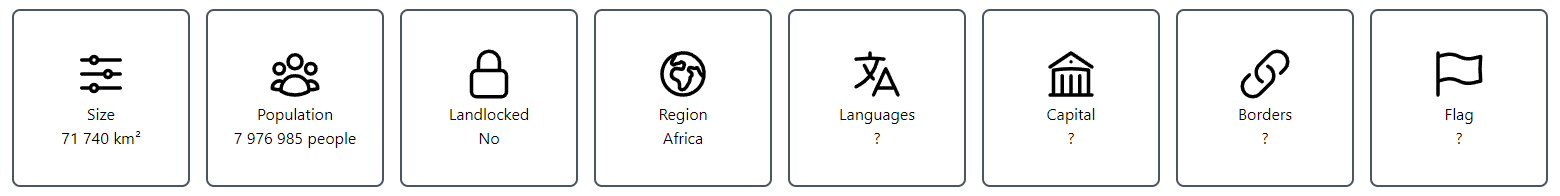
\includegraphics[width=.97\textwidth]{images/HintBoxes.jpg}
	\caption[HintBoxes]{HintBoxes - vlastní zpracování}
	\label{fig:reacthintboxes}
\end{figure}

Klíčová komponenta CountryGuessInput, kterou definujeme uvnitř souboru \emph{CountryGuessInput.tsx}, umožní uživateli zadat svůj tip. 
Začneme s~JSX, kde vytvoříme formulářový prvek pro zadání názvu země, potvrzovací tlačítko a~podmenu textového pole, které zobrazí nejpodobnější země na základě zadaného textu (filtrované země). 
Přidáme obslužné funkce pro akce a~události nad formulářem, které následně doimplementujeme.

\begin{figure}[htb]
	\centering
		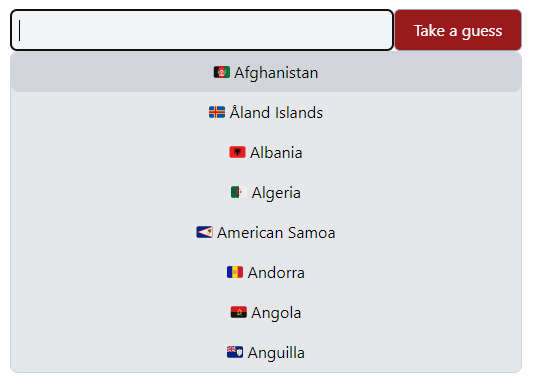
\includegraphics[width=.5\textwidth]{images/CountryGuessInput.jpg}
	\caption[CountryGuessInput]{CountryGuessInput - vlastní zpracování}
	\label{fig:reactcountryguessinput}
\end{figure}

V~komponentě, na základě vstupu \emph{countries}, získáme pole všech zemí bez těch, které uživatel již hádal (\emph{countriesWithoutAlreadyGuessed}). Poté definujeme a~inicializujeme ostatní stavy. 
Při kliknutí na tlačíko se zavolá funkce \emph{handleGuessButtonClick}, která volá obslužnou funkci \emph{handleEvaluateGuessAndUpdateState} v~rodičovské komponentě a~také funkci \emph{handleChangeSelectedGuess}. 
Funkce \emph{handleChangeSelectedGuess} aktualizuje aktuální tip, filtrované země a~uzavře podmenu. Funkce \emph{handleInputChange} převede tip uživatele do daného formátu, poté aktualizuje aktuální tip a~filtrované země. 
Ovládání formulářového prvku pomocí klávesnice umožní funkce \emph{handleKeyDown}.

Pomocná funkce \emph{updateGuessAndFilteredCountries} získá aktuálně filtrované země na základě uživatelova tipu. Následně aktualizuje stavy \emph{currentGuess}, \emph{isValidGuess} a~\emph{filteredCountries}. 
Funkce \emph{clampSelectedGuessIndex} zajistí, aby index uživatelem vybrané země byl v~požadovaném rozmezí (0 až počet filtrovaných zemí). 
Pro aktualizaci vlastnosti \emph{selectedGuessIndex} slouží funkce \emph{changeSelectedGuessIndex}, která index aktualizuje o~hodnotu předanou v~argumentu.
V~neposlední řadě funkce \emph{convertToFormattedGuess} převede tip uživatele tak, aby začínal velkým písmenem a~zbytek řetezce byl složen z~malých písmen.

Pro zobrazení všech doposud hádaných zemí uživatelem vytvoříme komponentu GuessedCountriesList. Ze vstupních vlastností \emph{countries}, \emph{guessedCountries} a~\emph{randomCountry} získáme proměnnou \emph{enrichedGuessedCountries}. 
Jde o~uživatelem hádané země s~vlajkou a~vzdáleností od \emph{randomCountry}. K~převodu využijeme JS funkce z~jiného souboru. 
Pro vypočtení vzdáleností použijeme knihovnu \emph{calculate-distance-between-coordinates} \cite{distancebetweencoordinates}, která obsahuje funkci \emph{getDistanceBetweenTwoPoints}. 
Jednotlivé prvky \emph{enrichedGuessedCountries} posléze vykreslíme v~JSX.

\begin{figure}[htb]
	\centering
		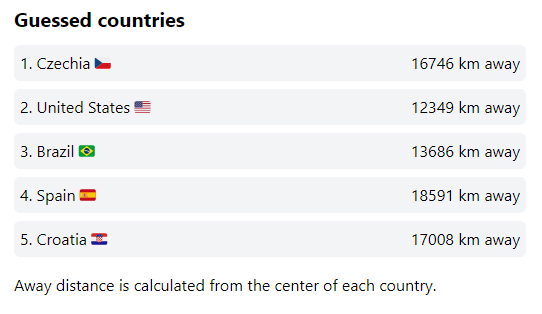
\includegraphics[width=.7\textwidth]{images/GuessedCountriesList.jpg}
	\caption[GuessedCountriesList]{GuessedCountriesList - vlastní zpracování}
	\label{fig:reactguessedcountrieslist}
\end{figure}

Nakonec vytvoříme modální okna, která se zobrazí při výhře či prohře. Stavy \emph{isWinModalOpen} a~\emph{isLoseModalOpen} aktualizujeme v~rámci funkce \emph{handleEvaluateGuessAndUpdateState} v~CountryGuesser. 
Na základě těchto stavů pak podmíněně vykreslíme daná modální okna. Oběma modálům předáme \emph{randomCountry} a~obslužnou funkci \emph{handleClose}. Výhernímu modálu také počet potřebných pokusů. 
V~jednotlivých komponentách (WinModal, LoseModal) vykreslíme komponentu BaseModal, která bude sloužit jako šablona pro obě okna. Do této komponenty vždy předáme titulek, obsah a~obslužnou funkci \emph{handleClose}. 
BaseModal následně v~JSX vykreslí základní strukturu modálního okna, s~dynamickými možnostmi pro titulek, obsah a~obslužnou funkci \emph{handleClose}.

\subsubsection*{Routování a layout aplikace}

Layout aplikace bude rozdělen do tří částí: hlavičky, patičky a~samotného obsahu, v~němž se vykreslí jednotlivé komponenty. Uživatel bude mít možnost přepínání mezi jednotlivými stránkami pomocí navigačního menu.

Pro routování využijeme knihovnu \emph{react-router-dom} \cite{reactrouter}. Začneme vytvořením souboru s~cestami (\emph{appRoutes}).

\begin{prog}
// Část souboru appRoutes.ts

interface AppRoute \{
  name: string;
  path: string;
  component: ComponentType;
  index?: boolean;
\}

export const appRoutes: ReadonlyArray<AppRoute> = [
  \{
    name: 'Home',
    path: '/',
    component: Landing,
    index: true,
  \},
  \{
    name: 'Counter',
    path: '/counter',
    component: Counter,
  \},
  // Další cesty...
];
\end{prog}

Následně v~kořeni aplikace vytvoříme \emph{router} pomocí předem definovaných cest aplikace. 
\emph{Router} vytvoříme díky dvěma pomocným funkcím k~tomu určených: \emph{createBrowserRouter} a~\emph{createRoutesFromElements}. 
Pokračujeme přiřazením proměnné \emph{router} do kořenové komponenty aplikace, konkrétně do poskytovatele \emph{RouterProvider}.

\begin{prog}
// Část souboru main.tsx

const router = createBrowserRouter(
  createRoutesFromElements(
    <Route path="/" element=\{<AppLayout />\} errorElement=\{<ErrorPage />\}>
      \{appRoutes.map(route => (
        <Route
          key=\{route.name\}
          index=\{route.index\}
          path=\{route.path\}
          Component=\{route.component\}
          caseSensitive
        />
      ))\}
    </Route>,
  ),
);

createRoot(document.getElementById('root')!).render(
  <StrictMode>
    <RouterProvider router=\{router\} />
  </StrictMode>,
);
\end{prog}

Hlavní komponenta AppLayout pak v~JSX vykreslí hlavičku, patičku a~dynamický obsah dle aktuální URL adresy, jenž vykreslí komponenta \emph{Outlet}.

\begin{prog}
// Část souboru AppLayout.tsx

function AppLayout() \{
  return (
    <div className="min-h-screen flex flex-col">
      <Header />

      <main className="flex-grow p-8">
        \{/* Outlet vykresluje šablonu (komponentu) pro aktuální URL adresu. */\}
        <Outlet />
      </main>

      <Footer />
    </div>
  );
\}
\end{prog}

V~hlavičce se budou nacházet odkazy na jednotlivé stránky. My se inspirujeme architekturou a~vzhledem navigačního menu Flowbite. 
Uvnitř komponenty Header vypíšeme všechny cesty aplikace pomocí komponenty \emph{NavLink} z~knihovny \emph{react-router-dom}. 
NavLink pomocí atributu \emph{className} umožňuje přistoupit k~vlastnosti \emph{isActive}, která indikuje, zda je cesta odkazu aktivní. 
Vlastnosti \emph{isActive} tedy využijeme pro podmíněné přidání CSS stylů. Pro korektní nastavení aria-current atributu, v~závislosti na aktuální URL, použijeme hook \emph{useLocation}, který vrací aktuální URL.

\begin{prog}
// Část souboru Header.tsx

\{appRoutes.map(route => (
  <li key=\{route.name\}>
    <NavLink
      to=\{route.path\}
      // react-router-dom poskytuje vlastnost "isActive"
        pro zvýraznění aktivního odkazu.
      className=\{(\{isActive\}) =>
        'block py-2 pr-4' +
        `\$\{
          isActive
            ? ' STATICKÉ STYLY PRO AKTIVNÍ ODKAZ...'
            : ' STATICKÉ STYLY PRO NEAKTIVNÍ ODKAZ...'
        \}`
      \}
      aria-current=\{route.path === currentPathName ? 'page' : undefined\}
    >
      \{route.name\}
    </NavLink>
  </li>
))\}
\end{prog}

Mobilní navigaci a~barevný režim implementujeme díky stavům \emph{isMobileNavOpen} a~\emph{isDarkMode}. Informaci o~tom, zda má uživatel zapnutý tmavý režim budeme ukládat do LocalStorage v~prohlížeči. 
K~tomu použijeme \emph{useEffect} hook, který při změně stavu \emph{isDarkMode} přidá patřičný data-mode a~provede aktualizaci LocalStorage.

\begin{prog}
// Část souboru Header.tsx

useEffect(() => \{
  if (isDarkMode) \{
    document.documentElement.setAttribute('data-mode', 'dark');
    localStorage.setItem('data-mode', 'dark');
  \} else \{
    document.documentElement.removeAttribute('data-mode');
    localStorage.removeItem('data-mode');
  \}
\}, [isDarkMode]);
\end{prog}